% Options for packages loaded elsewhere
\PassOptionsToPackage{unicode}{hyperref}
\PassOptionsToPackage{hyphens}{url}
\documentclass[
]{book}
\usepackage{xcolor}
\usepackage{amsmath,amssymb}
\setcounter{secnumdepth}{5}
\usepackage{iftex}
\ifPDFTeX
  \usepackage[T1]{fontenc}
  \usepackage[utf8]{inputenc}
  \usepackage{textcomp} % provide euro and other symbols
\else % if luatex or xetex
  \usepackage{unicode-math} % this also loads fontspec
  \defaultfontfeatures{Scale=MatchLowercase}
  \defaultfontfeatures[\rmfamily]{Ligatures=TeX,Scale=1}
\fi
\usepackage{lmodern}
\ifPDFTeX\else
  % xetex/luatex font selection
\fi
% Use upquote if available, for straight quotes in verbatim environments
\IfFileExists{upquote.sty}{\usepackage{upquote}}{}
\IfFileExists{microtype.sty}{% use microtype if available
  \usepackage[]{microtype}
  \UseMicrotypeSet[protrusion]{basicmath} % disable protrusion for tt fonts
}{}
\makeatletter
\@ifundefined{KOMAClassName}{% if non-KOMA class
  \IfFileExists{parskip.sty}{%
    \usepackage{parskip}
  }{% else
    \setlength{\parindent}{0pt}
    \setlength{\parskip}{6pt plus 2pt minus 1pt}}
}{% if KOMA class
  \KOMAoptions{parskip=half}}
\makeatother
\usepackage{color}
\usepackage{fancyvrb}
\newcommand{\VerbBar}{|}
\newcommand{\VERB}{\Verb[commandchars=\\\{\}]}
\DefineVerbatimEnvironment{Highlighting}{Verbatim}{commandchars=\\\{\}}
% Add ',fontsize=\small' for more characters per line
\usepackage{framed}
\definecolor{shadecolor}{RGB}{248,248,248}
\newenvironment{Shaded}{\begin{snugshade}}{\end{snugshade}}
\newcommand{\AlertTok}[1]{\textcolor[rgb]{0.94,0.16,0.16}{#1}}
\newcommand{\AnnotationTok}[1]{\textcolor[rgb]{0.56,0.35,0.01}{\textbf{\textit{#1}}}}
\newcommand{\AttributeTok}[1]{\textcolor[rgb]{0.13,0.29,0.53}{#1}}
\newcommand{\BaseNTok}[1]{\textcolor[rgb]{0.00,0.00,0.81}{#1}}
\newcommand{\BuiltInTok}[1]{#1}
\newcommand{\CharTok}[1]{\textcolor[rgb]{0.31,0.60,0.02}{#1}}
\newcommand{\CommentTok}[1]{\textcolor[rgb]{0.56,0.35,0.01}{\textit{#1}}}
\newcommand{\CommentVarTok}[1]{\textcolor[rgb]{0.56,0.35,0.01}{\textbf{\textit{#1}}}}
\newcommand{\ConstantTok}[1]{\textcolor[rgb]{0.56,0.35,0.01}{#1}}
\newcommand{\ControlFlowTok}[1]{\textcolor[rgb]{0.13,0.29,0.53}{\textbf{#1}}}
\newcommand{\DataTypeTok}[1]{\textcolor[rgb]{0.13,0.29,0.53}{#1}}
\newcommand{\DecValTok}[1]{\textcolor[rgb]{0.00,0.00,0.81}{#1}}
\newcommand{\DocumentationTok}[1]{\textcolor[rgb]{0.56,0.35,0.01}{\textbf{\textit{#1}}}}
\newcommand{\ErrorTok}[1]{\textcolor[rgb]{0.64,0.00,0.00}{\textbf{#1}}}
\newcommand{\ExtensionTok}[1]{#1}
\newcommand{\FloatTok}[1]{\textcolor[rgb]{0.00,0.00,0.81}{#1}}
\newcommand{\FunctionTok}[1]{\textcolor[rgb]{0.13,0.29,0.53}{\textbf{#1}}}
\newcommand{\ImportTok}[1]{#1}
\newcommand{\InformationTok}[1]{\textcolor[rgb]{0.56,0.35,0.01}{\textbf{\textit{#1}}}}
\newcommand{\KeywordTok}[1]{\textcolor[rgb]{0.13,0.29,0.53}{\textbf{#1}}}
\newcommand{\NormalTok}[1]{#1}
\newcommand{\OperatorTok}[1]{\textcolor[rgb]{0.81,0.36,0.00}{\textbf{#1}}}
\newcommand{\OtherTok}[1]{\textcolor[rgb]{0.56,0.35,0.01}{#1}}
\newcommand{\PreprocessorTok}[1]{\textcolor[rgb]{0.56,0.35,0.01}{\textit{#1}}}
\newcommand{\RegionMarkerTok}[1]{#1}
\newcommand{\SpecialCharTok}[1]{\textcolor[rgb]{0.81,0.36,0.00}{\textbf{#1}}}
\newcommand{\SpecialStringTok}[1]{\textcolor[rgb]{0.31,0.60,0.02}{#1}}
\newcommand{\StringTok}[1]{\textcolor[rgb]{0.31,0.60,0.02}{#1}}
\newcommand{\VariableTok}[1]{\textcolor[rgb]{0.00,0.00,0.00}{#1}}
\newcommand{\VerbatimStringTok}[1]{\textcolor[rgb]{0.31,0.60,0.02}{#1}}
\newcommand{\WarningTok}[1]{\textcolor[rgb]{0.56,0.35,0.01}{\textbf{\textit{#1}}}}
\usepackage{longtable,booktabs,array}
\usepackage{calc} % for calculating minipage widths
% Correct order of tables after \paragraph or \subparagraph
\usepackage{etoolbox}
\makeatletter
\patchcmd\longtable{\par}{\if@noskipsec\mbox{}\fi\par}{}{}
\makeatother
% Allow footnotes in longtable head/foot
\IfFileExists{footnotehyper.sty}{\usepackage{footnotehyper}}{\usepackage{footnote}}
\makesavenoteenv{longtable}
\usepackage{graphicx}
\makeatletter
\newsavebox\pandoc@box
\newcommand*\pandocbounded[1]{% scales image to fit in text height/width
  \sbox\pandoc@box{#1}%
  \Gscale@div\@tempa{\textheight}{\dimexpr\ht\pandoc@box+\dp\pandoc@box\relax}%
  \Gscale@div\@tempb{\linewidth}{\wd\pandoc@box}%
  \ifdim\@tempb\p@<\@tempa\p@\let\@tempa\@tempb\fi% select the smaller of both
  \ifdim\@tempa\p@<\p@\scalebox{\@tempa}{\usebox\pandoc@box}%
  \else\usebox{\pandoc@box}%
  \fi%
}
% Set default figure placement to htbp
\def\fps@figure{htbp}
\makeatother
\setlength{\emergencystretch}{3em} % prevent overfull lines
\providecommand{\tightlist}{%
  \setlength{\itemsep}{0pt}\setlength{\parskip}{0pt}}
\usepackage[]{natbib}
\bibliographystyle{apalike}
\usepackage{booktabs}
\usepackage{amsthm}
\makeatletter
\def\thm@space@setup{%
  \thm@preskip=8pt plus 2pt minus 4pt
  \thm@postskip=\thm@preskip
}
\makeatother
\usepackage{bookmark}
\IfFileExists{xurl.sty}{\usepackage{xurl}}{} % add URL line breaks if available
\urlstyle{same}
\hypersetup{
  pdftitle={A Minimal Book Example},
  pdfauthor={Yihui Xie},
  hidelinks,
  pdfcreator={LaTeX via pandoc}}

\title{A Minimal Book Example}
\author{Yihui Xie}
\date{2026-08-06}

\begin{document}
\maketitle

{
\setcounter{tocdepth}{1}
\tableofcontents
}
\chapter{Prerequisites}\label{prerequisites}

This is a \emph{sample} book written in \textbf{Markdown}. You can use anything that Pandoc's Markdown supports, e.g., a math equation \(a^2 + b^2 = c^2\).

The \textbf{bookdown} package can be installed from CRAN or Github:

\begin{Shaded}
\begin{Highlighting}[]
\FunctionTok{install.packages}\NormalTok{(}\StringTok{"bookdown"}\NormalTok{)}
\CommentTok{\# or the development version}
\CommentTok{\# devtools::install\_github("rstudio/bookdown")}
\end{Highlighting}
\end{Shaded}

Remember each Rmd file contains one and only one chapter, and a chapter is defined by the first-level heading \texttt{\#}.

To compile this example to PDF, you need XeLaTeX. You are recommended to install TinyTeX (which includes XeLaTeX): \url{https://yihui.org/tinytex/}.

\chapter{Introduction}\label{intro}

\begin{Shaded}
\begin{Highlighting}[]
\FunctionTok{library}\NormalTok{(tidyverse)}
\end{Highlighting}
\end{Shaded}

\begin{verbatim}
## -- Attaching core tidyverse packages ------------------------ tidyverse 2.0.0 --
## v dplyr     1.2.1     v readr     2.2.0
## v forcats   1.0.1     v stringr   1.6.0
## v ggplot2   4.0.3     v tibble    3.3.1
## v lubridate 1.9.5     v tidyr     1.3.2
## v purrr     1.2.2     
## -- Conflicts ------------------------------------------ tidyverse_conflicts() --
## x dplyr::filter() masks stats::filter()
## x dplyr::lag()    masks stats::lag()
## i Use the conflicted package (<http://conflicted.r-lib.org/>) to force all conflicts to become errors
\end{verbatim}

\begin{Shaded}
\begin{Highlighting}[]
\FunctionTok{library}\NormalTok{(Amelia)}
\end{Highlighting}
\end{Shaded}

\begin{verbatim}
## Cargando paquete requerido: Rcpp
## ## 
## ## Amelia II: Multiple Imputation
## ## (Version 1.8.3, built: 2024-11-07)
## ## Copyright (C) 2005-2026 James Honaker, Gary King and Matthew Blackwell
## ## Refer to http://gking.harvard.edu/amelia/ for more information
## ##
\end{verbatim}

\begin{Shaded}
\begin{Highlighting}[]
\FunctionTok{library}\NormalTok{(moments)}
\FunctionTok{library}\NormalTok{(patchwork)}
\FunctionTok{library}\NormalTok{(GGally)}
\end{Highlighting}
\end{Shaded}

Carguemos el conjunto de datos:

\begin{Shaded}
\begin{Highlighting}[]
\NormalTok{url }\OtherTok{\textless{}{-}} \StringTok{"https://raw.githubusercontent.com/cdeoroaguado/Datos/main/dataml/housing.csv"}
\NormalTok{datos }\OtherTok{\textless{}{-}} \FunctionTok{read.csv}\NormalTok{(url)}
\end{Highlighting}
\end{Shaded}

Verifiquemos que leímos bien los datos viendo el encabezado y la cola de los datos:

\begin{Shaded}
\begin{Highlighting}[]
\FunctionTok{head}\NormalTok{(datos,}\AttributeTok{n=}\DecValTok{5}\NormalTok{)}
\end{Highlighting}
\end{Shaded}

\begin{verbatim}
##   longitude latitude housing_median_age total_rooms total_bedrooms population
## 1   -122.23    37.88                 41         880            129        322
## 2   -122.22    37.86                 21        7099           1106       2401
## 3   -122.24    37.85                 52        1467            190        496
## 4   -122.25    37.85                 52        1274            235        558
## 5   -122.25    37.85                 52        1627            280        565
##   households median_income median_house_value ocean_proximity
## 1        126        8.3252             452600        NEAR BAY
## 2       1138        8.3014             358500        NEAR BAY
## 3        177        7.2574             352100        NEAR BAY
## 4        219        5.6431             341300        NEAR BAY
## 5        259        3.8462             342200        NEAR BAY
\end{verbatim}

Las dimensiones, los nombres de las columnas y la estructura de la base de datos se obtienen con los códigos:

\begin{Shaded}
\begin{Highlighting}[]
\FunctionTok{dim}\NormalTok{(datos)}
\end{Highlighting}
\end{Shaded}

\begin{verbatim}
## [1] 20640    10
\end{verbatim}

\begin{Shaded}
\begin{Highlighting}[]
\FunctionTok{colnames}\NormalTok{(datos)}
\end{Highlighting}
\end{Shaded}

\begin{verbatim}
##  [1] "longitude"          "latitude"           "housing_median_age"
##  [4] "total_rooms"        "total_bedrooms"     "population"        
##  [7] "households"         "median_income"      "median_house_value"
## [10] "ocean_proximity"
\end{verbatim}

\begin{Shaded}
\begin{Highlighting}[]
\FunctionTok{str}\NormalTok{(datos)}
\end{Highlighting}
\end{Shaded}

\begin{verbatim}
## 'data.frame':    20640 obs. of  10 variables:
##  $ longitude         : num  -122 -122 -122 -122 -122 ...
##  $ latitude          : num  37.9 37.9 37.9 37.9 37.9 ...
##  $ housing_median_age: num  41 21 52 52 52 52 52 52 42 52 ...
##  $ total_rooms       : num  880 7099 1467 1274 1627 ...
##  $ total_bedrooms    : num  129 1106 190 235 280 ...
##  $ population        : num  322 2401 496 558 565 ...
##  $ households        : num  126 1138 177 219 259 ...
##  $ median_income     : num  8.33 8.3 7.26 5.64 3.85 ...
##  $ median_house_value: num  452600 358500 352100 341300 342200 ...
##  $ ocean_proximity   : chr  "NEAR BAY" "NEAR BAY" "NEAR BAY" "NEAR BAY" ...
\end{verbatim}

Identifiquemos los valores NA por columna:

\begin{Shaded}
\begin{Highlighting}[]
\NormalTok{df }\OtherTok{\textless{}{-}}\NormalTok{ datos}

\NormalTok{df }\SpecialCharTok{\%\textgreater{}\%}
    \FunctionTok{summarise}\NormalTok{(}\FunctionTok{across}\NormalTok{(}\FunctionTok{everything}\NormalTok{(), }\SpecialCharTok{\textasciitilde{}} \FunctionTok{sum}\NormalTok{(}\FunctionTok{is.na}\NormalTok{(.)), }\AttributeTok{.names =} \StringTok{"NA\_\{.col\}"}\NormalTok{))}
\end{Highlighting}
\end{Shaded}

\begin{verbatim}
##   NA_longitude NA_latitude NA_housing_median_age NA_total_rooms
## 1            0           0                     0              0
##   NA_total_bedrooms NA_population NA_households NA_median_income
## 1               207             0             0                0
##   NA_median_house_value NA_ocean_proximity
## 1                     0                  0
\end{verbatim}

Como tenemos valores ausentes lo vamos a llenar con el promedio:

\begin{Shaded}
\begin{Highlighting}[]
\NormalTok{df }\OtherTok{\textless{}{-}}\NormalTok{ df }\SpecialCharTok{\%\textgreater{}\%}
  \FunctionTok{mutate}\NormalTok{(}
    \FunctionTok{across}\NormalTok{(}
      \FunctionTok{where}\NormalTok{(is.numeric),}
      \SpecialCharTok{\textasciitilde{}} \FunctionTok{ifelse}\NormalTok{(}\FunctionTok{is.na}\NormalTok{(.), }\FunctionTok{mean}\NormalTok{(., }\AttributeTok{na.rm =} \ConstantTok{TRUE}\NormalTok{), .)}
\NormalTok{    )}
\NormalTok{  )}
\end{Highlighting}
\end{Shaded}

Verifiquemos si fueron llenados con el promedio:

\begin{Shaded}
\begin{Highlighting}[]
\NormalTok{df }\SpecialCharTok{\%\textgreater{}\%}
  \FunctionTok{summarise}\NormalTok{(}\FunctionTok{across}\NormalTok{(}\FunctionTok{everything}\NormalTok{(), }\SpecialCharTok{\textasciitilde{}} \FunctionTok{sum}\NormalTok{(}\FunctionTok{is.na}\NormalTok{(.)), }\AttributeTok{.names =} \StringTok{"NA\_\{.col\}"}\NormalTok{))}
\end{Highlighting}
\end{Shaded}

\begin{verbatim}
##   NA_longitude NA_latitude NA_housing_median_age NA_total_rooms
## 1            0           0                     0              0
##   NA_total_bedrooms NA_population NA_households NA_median_income
## 1                 0             0             0                0
##   NA_median_house_value NA_ocean_proximity
## 1                     0                  0
\end{verbatim}

\section{\texorpdfstring{Analisis exploratorio de \texttt{median\_house\_value}}{Analisis exploratorio de median\_house\_value}}\label{analisis-exploratorio-de-median_house_value}

(Target)

Realicemos el resumen estadístico de la variable

\begin{Shaded}
\begin{Highlighting}[]
\NormalTok{df }\SpecialCharTok{\%\textgreater{}\%} \FunctionTok{summarise}\NormalTok{ (}\AttributeTok{n =} \FunctionTok{length}\NormalTok{(median\_house\_value),}
                  \AttributeTok{media =} \FunctionTok{mean}\NormalTok{(median\_house\_value),}
                  \AttributeTok{sd =} \FunctionTok{sd}\NormalTok{(median\_house\_value),}
                  \AttributeTok{mediana =} \FunctionTok{median}\NormalTok{(median\_house\_value),}
                  \AttributeTok{RIC =} \FunctionTok{IQR}\NormalTok{(median\_house\_value),}
                  \AttributeTok{Q1 =} \FunctionTok{quantile}\NormalTok{(median\_house\_value,}\FloatTok{0.25}\NormalTok{),}
                  \AttributeTok{Q3 =} \FunctionTok{quantile}\NormalTok{(median\_house\_value,}\FloatTok{0.75}\NormalTok{),}
                  \AttributeTok{minimo =} \FunctionTok{min}\NormalTok{(median\_house\_value),}
                  \AttributeTok{maximo =} \FunctionTok{max}\NormalTok{(median\_house\_value),}
                  \AttributeTok{curtosis =} \FunctionTok{kurtosis}\NormalTok{(median\_house\_value),}
                  \AttributeTok{asimetria =} \FunctionTok{skewness}\NormalTok{(median\_house\_value))}
\end{Highlighting}
\end{Shaded}

\begin{verbatim}
##       n    media       sd mediana    RIC     Q1     Q3 minimo maximo curtosis
## 1 20640 206855.8 115395.6  179700 145125 119600 264725  14999 500001   3.3275
##   asimetria
## 1 0.9776922
\end{verbatim}

Veamos un histograma:

\begin{Shaded}
\begin{Highlighting}[]
\NormalTok{df }\SpecialCharTok{\%\textgreater{}\%}
  \FunctionTok{ggplot}\NormalTok{(}\FunctionTok{aes}\NormalTok{(}\AttributeTok{x =}\NormalTok{ median\_house\_value)) }\SpecialCharTok{+}
  \FunctionTok{geom\_histogram}\NormalTok{(}\FunctionTok{aes}\NormalTok{(}\AttributeTok{y =} \FunctionTok{after\_stat}\NormalTok{(density)), }
                 \AttributeTok{binwidth =} \DecValTok{25000}\NormalTok{, }
                 \AttributeTok{fill =} \StringTok{"\#F598C4"}\NormalTok{, }
                 \AttributeTok{color =} \StringTok{"white"}\NormalTok{, }
                 \AttributeTok{alpha =} \FloatTok{0.6}\NormalTok{) }\SpecialCharTok{+}
  \FunctionTok{geom\_density}\NormalTok{(}\AttributeTok{color =} \StringTok{"\#3D9970"}\NormalTok{, }\AttributeTok{linewidth =} \FloatTok{1.2}\NormalTok{) }\SpecialCharTok{+}
  \FunctionTok{labs}\NormalTok{(}
    \AttributeTok{title =} \StringTok{"Distribución del valor medio de las viviendas"}\NormalTok{,}
    \AttributeTok{x =} \StringTok{"Valor medio de la vivienda (USD)"}\NormalTok{,}
    \AttributeTok{y =} \StringTok{"Densidad"}
\NormalTok{  ) }\SpecialCharTok{+}
  \FunctionTok{theme\_bw}\NormalTok{()}
\end{Highlighting}
\end{Shaded}

\pandocbounded{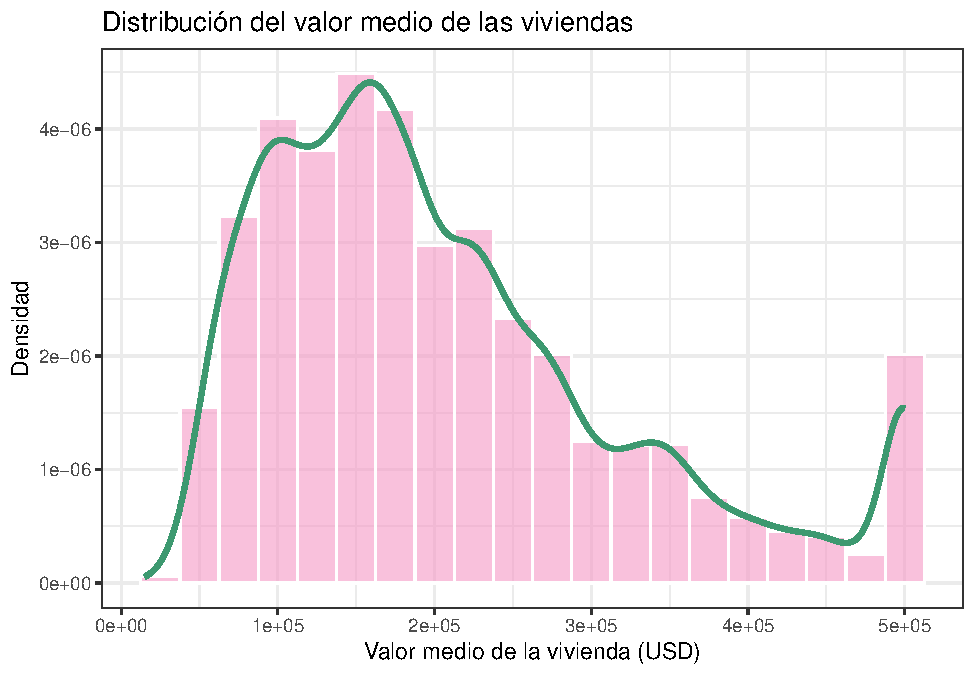
\includegraphics[keepaspectratio]{bookdown-demo_files/bookdown-demo_files/figure-latex/histhousevalue-1.pdf}}
Veamos un diagrama de cajas y bigotes:

\begin{Shaded}
\begin{Highlighting}[]
\NormalTok{df }\SpecialCharTok{\%\textgreater{}\%}
  \FunctionTok{ggplot}\NormalTok{(}\FunctionTok{aes}\NormalTok{(}\AttributeTok{x =} \StringTok{""}\NormalTok{, }\AttributeTok{y =}\NormalTok{ median\_house\_value)) }\SpecialCharTok{+}
  \FunctionTok{geom\_boxplot}\NormalTok{(}\AttributeTok{fill =} \StringTok{"lightblue"}\NormalTok{, }\AttributeTok{color =} \StringTok{"darkblue"}\NormalTok{, }\AttributeTok{outlier.color =} \StringTok{"darkred"}\NormalTok{) }\SpecialCharTok{+}
  \FunctionTok{stat\_summary}\NormalTok{(}
    \AttributeTok{fun =}\NormalTok{ mean,}
    \AttributeTok{geom =} \StringTok{"point"}\NormalTok{,}
    \AttributeTok{shape =} \DecValTok{20}\NormalTok{,}
    \AttributeTok{size =} \DecValTok{3}\NormalTok{,}
    \AttributeTok{color =} \StringTok{"black"}
\NormalTok{  ) }\SpecialCharTok{+}
  \FunctionTok{labs}\NormalTok{(}
    \AttributeTok{title =} \StringTok{"Diagrama de cajas y bigotes del valor medio de las viviendas"}\NormalTok{,}
    \AttributeTok{x =} \StringTok{""}\NormalTok{,}
    \AttributeTok{y =} \StringTok{"Valor medio de la vivienda (USD)"}
\NormalTok{  ) }\SpecialCharTok{+}
  \FunctionTok{theme\_bw}\NormalTok{()}
\end{Highlighting}
\end{Shaded}

\pandocbounded{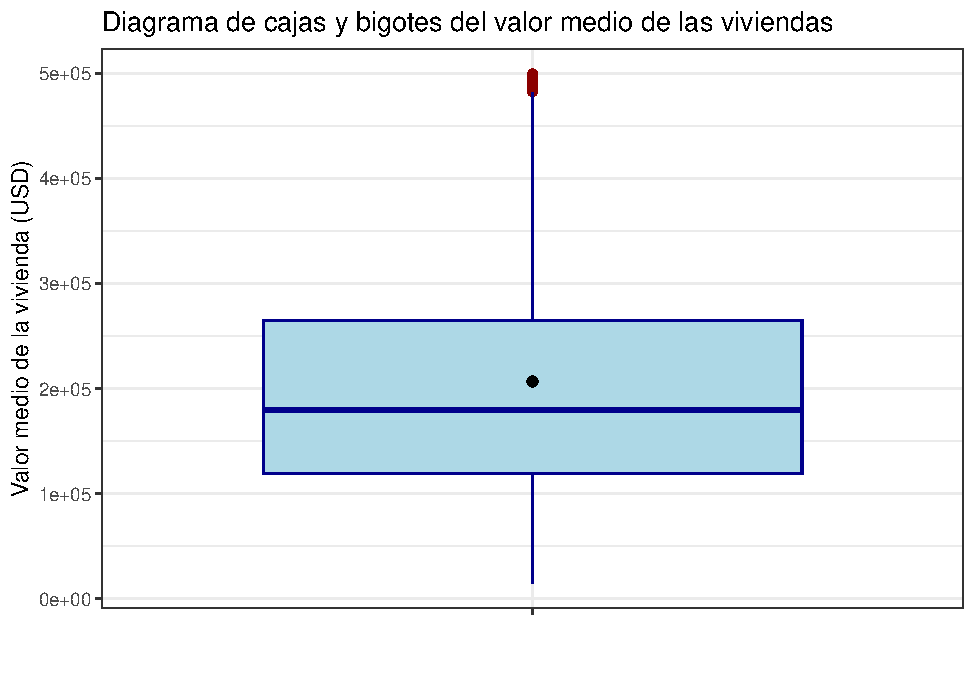
\includegraphics[keepaspectratio]{bookdown-demo_files/bookdown-demo_files/figure-latex/boxplotvaluehouse-1.pdf}}

\begin{Shaded}
\begin{Highlighting}[]
\NormalTok{df }\SpecialCharTok{\%\textgreater{}\%}
  \FunctionTok{select}\NormalTok{(}\FunctionTok{where}\NormalTok{(is.numeric), }\SpecialCharTok{{-}}\NormalTok{median\_house\_value) }\SpecialCharTok{\%\textgreater{}\%}
  \FunctionTok{pivot\_longer}\NormalTok{(}
    \AttributeTok{cols =} \FunctionTok{everything}\NormalTok{(),}
    \AttributeTok{names\_to =} \StringTok{\textquotesingle{}variable\textquotesingle{}}\NormalTok{,}
    \AttributeTok{values\_to =} \StringTok{\textquotesingle{}valor\textquotesingle{}}
\NormalTok{  ) }\SpecialCharTok{\%\textgreater{}\%}
  \FunctionTok{group\_by}\NormalTok{(variable) }\SpecialCharTok{\%\textgreater{}\%}
  \FunctionTok{summarise}\NormalTok{(}\AttributeTok{n =} \FunctionTok{length}\NormalTok{(valor),}
                \AttributeTok{media =} \FunctionTok{mean}\NormalTok{(valor),}
                \AttributeTok{sd =} \FunctionTok{sd}\NormalTok{(valor),}
                \AttributeTok{mediana =} \FunctionTok{median}\NormalTok{(valor),}
                \AttributeTok{RIC =} \FunctionTok{IQR}\NormalTok{(valor),}
                \AttributeTok{Q1 =} \FunctionTok{quantile}\NormalTok{(valor,}\FloatTok{0.25}\NormalTok{),}
                \AttributeTok{Q3 =} \FunctionTok{quantile}\NormalTok{(valor,}\FloatTok{0.75}\NormalTok{),}
                \AttributeTok{minimo =} \FunctionTok{min}\NormalTok{(valor),}
                \AttributeTok{maximo =} \FunctionTok{max}\NormalTok{(valor),}
                \AttributeTok{curtosis =} \FunctionTok{kurtosis}\NormalTok{(valor),}
                \AttributeTok{asimetria =} \FunctionTok{skewness}\NormalTok{(valor)}
\NormalTok{              )}
\end{Highlighting}
\end{Shaded}

\begin{verbatim}
## # A tibble: 8 x 12
##   variable      n   media     sd mediana    RIC      Q1      Q3   minimo  maximo
##   <chr>     <int>   <dbl>  <dbl>   <dbl>  <dbl>   <dbl>   <dbl>    <dbl>   <dbl>
## 1 househol~ 20640  500.   3.82e2  409    3.25e2  280     605       1      6082  
## 2 housing_~ 20640   28.6  1.26e1   29    1.9 e1   18      37       1        52  
## 3 latitude  20640   35.6  2.14e0   34.3  3.78e0   33.9    37.7    32.5      42.0
## 4 longitude 20640 -120.   2.00e0 -118.   3.79e0 -122.   -118.   -124.     -114. 
## 5 median_i~ 20640    3.87 1.90e0    3.53 2.18e0    2.56    4.74    0.500    15.0
## 6 populati~ 20640 1425.   1.13e3 1166    9.38e2  787    1725       3     35682  
## 7 total_be~ 20640  538.   4.19e2  438    3.46e2  297     643.      1      6445  
## 8 total_ro~ 20640 2636.   2.18e3 2127    1.70e3 1448.   3148       2     39320  
## # i 2 more variables: curtosis <dbl>, asimetria <dbl>
\end{verbatim}

\begin{Shaded}
\begin{Highlighting}[]
\NormalTok{resumen\_numericas }\OtherTok{\textless{}{-}}\NormalTok{ df }\SpecialCharTok{\%\textgreater{}\%}
  \FunctionTok{select}\NormalTok{(}\FunctionTok{where}\NormalTok{(is.numeric), }\SpecialCharTok{{-}}\NormalTok{median\_house\_value) }\SpecialCharTok{\%\textgreater{}\%}
  \FunctionTok{pivot\_longer}\NormalTok{(}
    \AttributeTok{cols =} \FunctionTok{everything}\NormalTok{(),}
    \AttributeTok{names\_to =} \StringTok{"variable"}\NormalTok{,}
    \AttributeTok{values\_to =} \StringTok{"valor"}
\NormalTok{  ) }\SpecialCharTok{\%\textgreater{}\%}
  \FunctionTok{group\_by}\NormalTok{(variable) }\SpecialCharTok{\%\textgreater{}\%}
  \FunctionTok{summarise}\NormalTok{(}
    \AttributeTok{n =} \FunctionTok{sum}\NormalTok{(}\SpecialCharTok{!}\FunctionTok{is.na}\NormalTok{(valor)),}
    \AttributeTok{media =} \FunctionTok{mean}\NormalTok{(valor, }\AttributeTok{na.rm =} \ConstantTok{TRUE}\NormalTok{),}
    \AttributeTok{ds =} \FunctionTok{sd}\NormalTok{(valor, }\AttributeTok{na.rm =} \ConstantTok{TRUE}\NormalTok{),}
    \AttributeTok{mediana =} \FunctionTok{median}\NormalTok{(valor, }\AttributeTok{na.rm =} \ConstantTok{TRUE}\NormalTok{),}
    \AttributeTok{minimo =} \FunctionTok{min}\NormalTok{(valor, }\AttributeTok{na.rm =} \ConstantTok{TRUE}\NormalTok{),}
    \AttributeTok{maximo =} \FunctionTok{max}\NormalTok{(valor, }\AttributeTok{na.rm =} \ConstantTok{TRUE}\NormalTok{),}
    \AttributeTok{Q1 =} \FunctionTok{quantile}\NormalTok{(valor, }\FloatTok{0.25}\NormalTok{, }\AttributeTok{na.rm =} \ConstantTok{TRUE}\NormalTok{),}
    \AttributeTok{Q3 =} \FunctionTok{quantile}\NormalTok{(valor, }\FloatTok{0.75}\NormalTok{, }\AttributeTok{na.rm =} \ConstantTok{TRUE}\NormalTok{),}
    \AttributeTok{IQR =} \FunctionTok{IQR}\NormalTok{(valor, }\AttributeTok{na.rm =} \ConstantTok{TRUE}\NormalTok{),}
    \AttributeTok{.groups =} \StringTok{"drop"}
\NormalTok{  )}

\NormalTok{resumen\_numericas}
\end{Highlighting}
\end{Shaded}

\begin{verbatim}
## # A tibble: 8 x 10
##   variable      n   media     ds mediana   minimo  maximo      Q1      Q3    IQR
##   <chr>     <int>   <dbl>  <dbl>   <dbl>    <dbl>   <dbl>   <dbl>   <dbl>  <dbl>
## 1 househol~ 20640  500.   3.82e2  409       1      6082    280     605    3.25e2
## 2 housing_~ 20640   28.6  1.26e1   29       1        52     18      37    1.9 e1
## 3 latitude  20640   35.6  2.14e0   34.3    32.5      42.0   33.9    37.7  3.78e0
## 4 longitude 20640 -120.   2.00e0 -118.   -124.     -114.  -122.   -118.   3.79e0
## 5 median_i~ 20640    3.87 1.90e0    3.53    0.500    15.0    2.56    4.74 2.18e0
## 6 populati~ 20640 1425.   1.13e3 1166       3     35682    787    1725    9.38e2
## 7 total_be~ 20640  538.   4.19e2  438       1      6445    297     643.   3.46e2
## 8 total_ro~ 20640 2636.   2.18e3 2127       2     39320   1448.   3148    1.70e3
\end{verbatim}

Ahora veamos la variable \texttt{ocean\_proximity}

\begin{Shaded}
\begin{Highlighting}[]
\NormalTok{df }\SpecialCharTok{\%\textgreater{}\%}
  \FunctionTok{count}\NormalTok{(ocean\_proximity, }\AttributeTok{name =} \StringTok{"n"}\NormalTok{) }\SpecialCharTok{\%\textgreater{}\%}
  \FunctionTok{mutate}\NormalTok{(}\AttributeTok{Porcentaje =} \FunctionTok{round}\NormalTok{((n}\SpecialCharTok{/}\FunctionTok{sum}\NormalTok{(n))}\SpecialCharTok{*}\DecValTok{100}\NormalTok{,}\DecValTok{2}\NormalTok{),}
         \AttributeTok{Variable =} \StringTok{\textquotesingle{}ocean\_proximity\textquotesingle{}}\NormalTok{,}
         \AttributeTok{Categoria =} \FunctionTok{as.character}\NormalTok{(ocean\_proximity)) }\SpecialCharTok{\%\textgreater{}\%} \FunctionTok{select}\NormalTok{(Variable,Categoria,n,Porcentaje) }\OtherTok{{-}\textgreater{}}\NormalTok{ tabla\_ocean}

\NormalTok{tabla\_ocean}
\end{Highlighting}
\end{Shaded}

\begin{verbatim}
##          Variable  Categoria    n Porcentaje
## 1 ocean_proximity  <1H OCEAN 9136      44.26
## 2 ocean_proximity     INLAND 6551      31.74
## 3 ocean_proximity     ISLAND    5       0.02
## 4 ocean_proximity   NEAR BAY 2290      11.09
## 5 ocean_proximity NEAR OCEAN 2658      12.88
\end{verbatim}

\begin{Shaded}
\begin{Highlighting}[]
\NormalTok{df }\SpecialCharTok{\%\textgreater{}\%}
  \FunctionTok{count}\NormalTok{(ocean\_proximity, }\AttributeTok{name =} \StringTok{"n"}\NormalTok{) }\SpecialCharTok{\%\textgreater{}\%}
  \FunctionTok{mutate}\NormalTok{(}\AttributeTok{Porcentaje =} \FunctionTok{round}\NormalTok{((n}\SpecialCharTok{/}\FunctionTok{sum}\NormalTok{(n))}\SpecialCharTok{*}\DecValTok{100}\NormalTok{,}\DecValTok{2}\NormalTok{),}
         \AttributeTok{Etiqueta =} \FunctionTok{paste0}\NormalTok{(n,}\StringTok{" ("}\NormalTok{,Porcentaje,}\StringTok{"\%)"}\NormalTok{)) }\OtherTok{{-}\textgreater{}}\NormalTok{ tabla\_ocean\_b}
\NormalTok{tabla\_ocean\_b }\SpecialCharTok{\%\textgreater{}\%}
  \FunctionTok{ggplot}\NormalTok{(}\FunctionTok{aes}\NormalTok{(}\AttributeTok{x =}\NormalTok{ ocean\_proximity, }\AttributeTok{y=}\NormalTok{n))}\SpecialCharTok{+}
  \FunctionTok{geom\_col}\NormalTok{(}\AttributeTok{fill =} \StringTok{"\#008B8B"}\NormalTok{, }\AttributeTok{width =} \FloatTok{0.6}\NormalTok{)}\SpecialCharTok{+}
  \FunctionTok{geom\_text}\NormalTok{(}\FunctionTok{aes}\NormalTok{(}\AttributeTok{label =}\NormalTok{ Etiqueta), }\AttributeTok{vjust=}\SpecialCharTok{{-}}\FloatTok{0.5}\NormalTok{, }\AttributeTok{size=}\FloatTok{4.5}\NormalTok{)}\SpecialCharTok{+}
  \FunctionTok{facet\_wrap}\NormalTok{(}\SpecialCharTok{\textasciitilde{}}\StringTok{\textquotesingle{}Distribución de la variable ocean proximity\textquotesingle{}}\NormalTok{)}\SpecialCharTok{+}
  \FunctionTok{scale\_y\_continuous}\NormalTok{(}\AttributeTok{expand =} \FunctionTok{expansion}\NormalTok{(}\AttributeTok{mult=}\FunctionTok{c}\NormalTok{(}\DecValTok{0}\NormalTok{,}\FloatTok{0.15}\NormalTok{)))}\SpecialCharTok{+}
  \FunctionTok{theme\_bw}\NormalTok{()}
\end{Highlighting}
\end{Shaded}

\pandocbounded{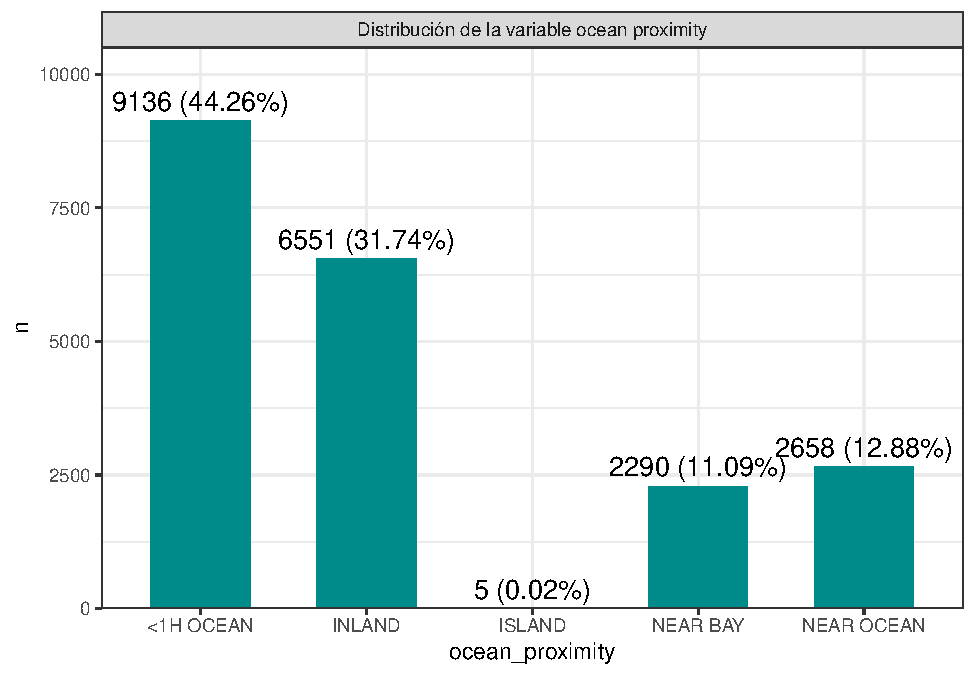
\includegraphics[keepaspectratio]{bookdown-demo_files/bookdown-demo_files/figure-latex/unnamed-chunk-5-1.pdf}}
\#\# Analisis exploratorio bivariado

\begin{Shaded}
\begin{Highlighting}[]
\NormalTok{df }\SpecialCharTok{\%\textgreater{}\%}
  \FunctionTok{ggplot}\NormalTok{(}\FunctionTok{aes}\NormalTok{(}\AttributeTok{x =}\NormalTok{ median\_income,}\AttributeTok{y=}\NormalTok{median\_house\_value))}\SpecialCharTok{+}
  \FunctionTok{geom\_point}\NormalTok{(}\AttributeTok{alpha=}\FloatTok{0.4}\NormalTok{, }\AttributeTok{color=}\StringTok{\textquotesingle{}darkblue\textquotesingle{}}\NormalTok{)}\SpecialCharTok{+}
  \FunctionTok{labs}\NormalTok{(}\AttributeTok{y=}\StringTok{\textquotesingle{}Valor medio de la vivienda\textquotesingle{}}\NormalTok{,}
       \AttributeTok{x=} \StringTok{\textquotesingle{}Ingreso medio\textquotesingle{}}\NormalTok{)}\SpecialCharTok{+}
  \FunctionTok{theme\_bw}\NormalTok{()}\SpecialCharTok{+}
  \FunctionTok{facet\_grid}\NormalTok{(.}\SpecialCharTok{\textasciitilde{}}\StringTok{\textquotesingle{}Dispersión entre el ingreso medio y el valor de la vivienda\textquotesingle{}}\NormalTok{)}
\end{Highlighting}
\end{Shaded}

\pandocbounded{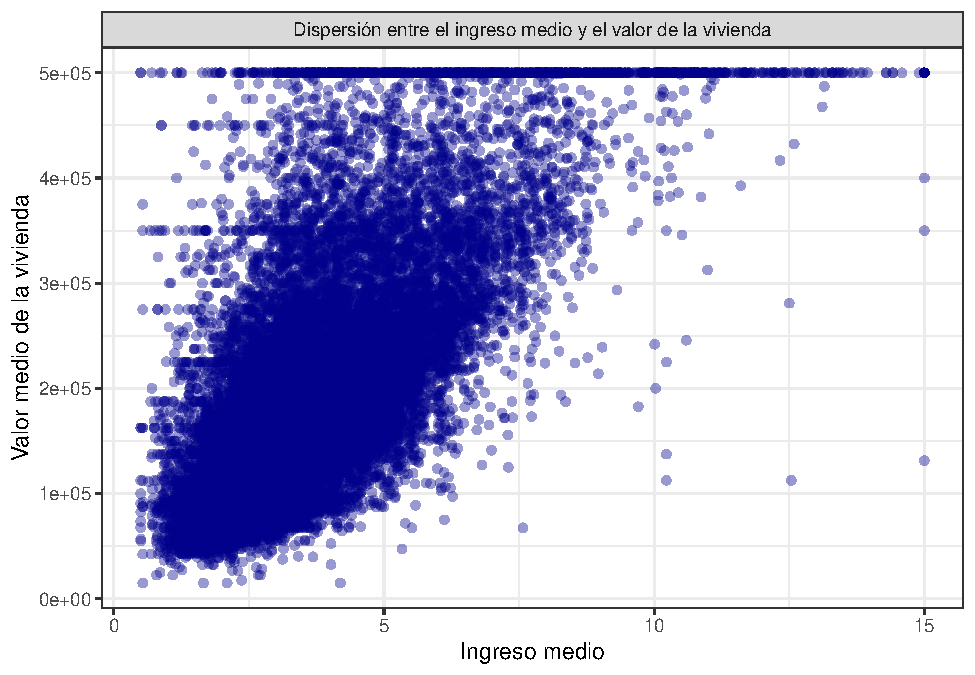
\includegraphics[keepaspectratio]{bookdown-demo_files/bookdown-demo_files/figure-latex/valorvsingreso-1.pdf}}

Ahora comparemos el valor medio de la vivienda según la proximidad al océano.

\begin{Shaded}
\begin{Highlighting}[]
\NormalTok{df }\SpecialCharTok{\%\textgreater{}\%} 
  \FunctionTok{group\_by}\NormalTok{(ocean\_proximity) }\SpecialCharTok{\%\textgreater{}\%} 
  \FunctionTok{summarise}\NormalTok{ (}\AttributeTok{n =} \FunctionTok{length}\NormalTok{(median\_house\_value),}
                  \AttributeTok{media =} \FunctionTok{mean}\NormalTok{(median\_house\_value),}
                  \AttributeTok{sd =} \FunctionTok{sd}\NormalTok{(median\_house\_value),}
                  \AttributeTok{mediana =} \FunctionTok{median}\NormalTok{(median\_house\_value),}
                  \AttributeTok{RIC =} \FunctionTok{IQR}\NormalTok{(median\_house\_value),}
                  \AttributeTok{Q1 =} \FunctionTok{quantile}\NormalTok{(median\_house\_value,}\FloatTok{0.25}\NormalTok{),}
                  \AttributeTok{Q3 =} \FunctionTok{quantile}\NormalTok{(median\_house\_value,}\FloatTok{0.75}\NormalTok{),}
                  \AttributeTok{minimo =} \FunctionTok{min}\NormalTok{(median\_house\_value),}
                  \AttributeTok{maximo =} \FunctionTok{max}\NormalTok{(median\_house\_value),}
                  \AttributeTok{curtosis =} \FunctionTok{kurtosis}\NormalTok{(median\_house\_value),}
                  \AttributeTok{asimetria =} \FunctionTok{skewness}\NormalTok{(median\_house\_value))}
\end{Highlighting}
\end{Shaded}

\begin{verbatim}
## # A tibble: 5 x 12
##   ocean_proximity     n  media     sd mediana    RIC     Q1     Q3 minimo maximo
##   <chr>           <int>  <dbl>  <dbl>   <dbl>  <dbl>  <dbl>  <dbl>  <dbl>  <dbl>
## 1 <1H OCEAN        9136 2.40e5 1.06e5  214850 125000 164100 289100  17500 500001
## 2 INLAND           6551 1.25e5 7.00e4  108500  71450  77500 148950  14999 500001
## 3 ISLAND              5 3.80e5 8.06e4  414700 150000 300000 450000 287500 450000
## 4 NEAR BAY         2290 2.59e5 1.23e5  233800 183200 162500 345700  22500 500001
## 5 NEAR OCEAN       2658 2.49e5 1.22e5  229450 172750 150000 322750  22500 500001
## # i 2 more variables: curtosis <dbl>, asimetria <dbl>
\end{verbatim}

veamos un gráfico de cajas y bigotes

\begin{Shaded}
\begin{Highlighting}[]
\NormalTok{df }\SpecialCharTok{\%\textgreater{}\%} 
  \FunctionTok{ggplot}\NormalTok{(}\FunctionTok{aes}\NormalTok{(}\AttributeTok{x=}\NormalTok{ocean\_proximity, }\AttributeTok{y=}\NormalTok{median\_house\_value))}\SpecialCharTok{+}
  \FunctionTok{geom\_boxplot}\NormalTok{()}
\end{Highlighting}
\end{Shaded}

\pandocbounded{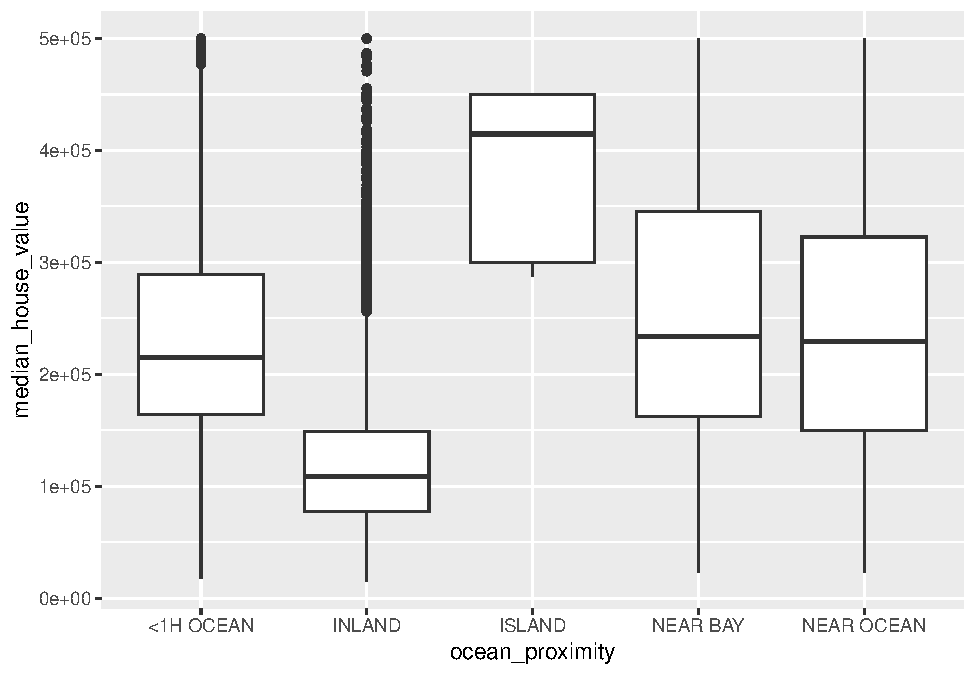
\includegraphics[keepaspectratio]{bookdown-demo_files/bookdown-demo_files/figure-latex/unnamed-chunk-6-1.pdf}}
\#\# Paquete GGally

\begin{Shaded}
\begin{Highlighting}[]
\NormalTok{ df }\SpecialCharTok{\%\textgreater{}\%}
  \FunctionTok{ggpairs}\NormalTok{()}
\end{Highlighting}
\end{Shaded}

\begin{verbatim}
## `stat_bin()` using `bins = 30`. Pick better value `binwidth`.
## `stat_bin()` using `bins = 30`. Pick better value `binwidth`.
## `stat_bin()` using `bins = 30`. Pick better value `binwidth`.
## `stat_bin()` using `bins = 30`. Pick better value `binwidth`.
## `stat_bin()` using `bins = 30`. Pick better value `binwidth`.
## `stat_bin()` using `bins = 30`. Pick better value `binwidth`.
## `stat_bin()` using `bins = 30`. Pick better value `binwidth`.
## `stat_bin()` using `bins = 30`. Pick better value `binwidth`.
## `stat_bin()` using `bins = 30`. Pick better value `binwidth`.
\end{verbatim}

\pandocbounded{
\includegraphics[keepaspectratio]{bookdown-demo_files/bookdown-demo_files/figure-latex/ggally-1.pdf}}

\chapter{Literature}\label{literature}

Here is a review of existing methods.

\chapter{Methods}\label{methods}

We describe our methods in this chapter.

Math can be added in body using usual syntax like this

\section{math example}\label{math-example}

\(p\) is unknown but expected to be around 1/3. Standard error will be approximated

\[
SE = \sqrt{\frac{p(1-p)}{n}} \approx \sqrt{\frac{1/3 (1 - 1/3)} {300}} = 0.027
\]

You can also use math in footnotes like this\footnote{where we mention \(p = \frac{a}{b}\)}.

We will approximate standard error to 0.027\footnote{\(p\) is unknown but expected to be around 1/3. Standard error will be approximated

  \[
  SE = \sqrt{\frac{p(1-p)}{n}} \approx \sqrt{\frac{1/3 (1 - 1/3)} {300}} = 0.027
  \]}

\chapter{Applications}\label{applications}

Some \emph{significant} applications are demonstrated in this chapter.

\section{Example one}\label{example-one}

\section{Example two}\label{example-two}

\chapter{Final Words}\label{final-words}

We have finished a nice book.

\bibliography{book.bib,packages.bib}

\end{document}
